%% Generelle Dokumenteigenschaften
\documentclass[a4paper, 12pt]{scrartcl}
\usepackage[T1]{fontenc}
\usepackage[german]{babel}
\usepackage[latin1]{inputenc}
\usepackage{ae,aecompl}
\newcommand{\p}{\paragraph{}}  %% neuer Absatz
\usepackage{german, a4, amsmath, amssymb, graphicx}
%\ifpdfoutput{%
%  \usepackage[pdftex]{graphicx}
%  \usepackage[pdftex,plainpages=false]{hyperref}
%  \pdfcompresslevel=9
%  \hypersetup{a4paper,pdftitle={CoMa - ein  Konferenz-Manager},pdfsubject={eine Spezifikation},pdfauthor={Sandro Esquivel, Tom Scherzer, Jan Waller},pdfborder=0}
%  \DeclareGraphicsExtensions{.jpg, .pdf, .mps, .png}
%}{%
%  \usepackage[plainpages=false]{hyperref}
%  \usepackage{graphicx}
%  \DeclareGraphicsExtensions{.eps}
%}

\begin{document}
%%%%%%%%%%%%%%%%%%%%%%%%%%%%%%%%%%%%%%%%%%%%%%%%%%%%%%%%%%%%%%%%%%
%%                                                              %%
%%                          Titelseite                          %%
%%                                                              %%
%%%%%%%%%%%%%%%%%%%%%%%%%%%%%%%%%%%%%%%%%%%%%%%%%%%%%%%%%%%%%%%%%%
\thispagestyle{empty}
\begin{center}
{\huge \bf \emph{CoMa - ein Konferenz-Manager}}

\vspace{2cm}

{\Large Auszug aus der Spezifikation - Das Datenmodell}

\vspace{2.25cm}


\includegraphics[width=5cm]{causiegel}

\vspace{2.25cm}

{\large
{\sc Christian-Albrechts-Universit\"{a}t zu Kiel} \\
Institut f\"{u}r Informatik und Praktische Mathematik \\
Lehrstuhl f\"{u}r Software-Technologie }

\vspace{2cm}

\begin{tabular}{ll}
ausgearbeitet von:           & {Sandro Esquivel} \\
                             & {Tom Scherzer} \\
                             & {Jan Waller} \\
\end{tabular}

\vspace{1cm}

Kiel, \today
\end{center}

\pagebreak

%%%%%%%%%%%%%%%%%%%%%%%%%%%%%%%%%%%%%%%%%%%%%%%%%%%%%%%%%%%%%%%%%%
%%                                                              %%
%%                       Text der Arbeit                        %%
%%                                                              %%
%%%%%%%%%%%%%%%%%%%%%%%%%%%%%%%%%%%%%%%%%%%%%%%%%%%%%%%%%%%%%%%%%%

\pagestyle{headings} \pagenumbering{arabic} \setcounter{page}{1}

    \section{Das Datenmodell f\"{u}r die Konferenz}

    \begin{tabular}{|c|}
      \hline
      \emph{Conference} \\
      \hline
      \underline{id} \\
      title \\
      description \\
      location \\
      time \\
      homepage \\
      \textbf{configuration:} \\
      submitPaperDeadline \\
      submitReviewDeadline \\
      minPapers, maxPapers \\
      \textbf{extended configuration:} \\
      topicNames* (\textit{common topics}) \\
      ratingCriteria* (\textit{common criteria}) \\
      ratingType (\textit{1: 1-5}) \\
      minReviewersPerPaper (\textit{3}) \\
      averageReviewersPerPaper (\textit{4}) \\
      criticalVariance (\textit{?}) \\
      autoValidateAccounts? (\textit{true}) \\
      autoStartPaperDiscussion? (\textit{true}) \\
      autoAddRereviewers? (\textit{false}) \\
      numRereviewers (\textit{2}) \\
      \hline
    \end{tabular}
    \begin{tabular}{|c|}
      \hline
      \emph{Person} \\
      \hline
      \underline{id} \\
      name \\
      address \\
      email \\
      phone \\
      description \\
      username \\
      password \\
      deleted? \\
      \hline
    \end{tabular}
    \begin{tabular}{c}
      \begin{tabular}{|c|}
        \hline
        \emph{Chair ($\rightarrow$ Person)} \\
        \hline
        \textit{none} \\
        \hline
      \end{tabular} \\
      \\
      \begin{tabular}{|c|}
        \hline
        \emph{Reviewer ($\rightarrow$ Person)} \\
        \hline
        $\longrightarrow$ papers* \\
        $\longrightarrow$ reviews* \\
        $\longrightarrow$ preferredTopics* \\
        \hline
      \end{tabular} \\
      \\
      \begin{tabular}{|c|}
        \hline
        \emph{Author ($\rightarrow$ Person)} \\
        \hline
        $\longrightarrow$ papers* \\
        \hline
      \end{tabular} \\
      \\
      \begin{tabular}{|c|}
        \hline
        \emph{Participant ($\rightarrow$ Person)} \\
        \hline
        \textit{none} \\
        \hline
      \end{tabular} \\
    \end{tabular} \\

    \begin{tabular}{|c|}
      \hline
      \emph{Paper} \\
      \hline
      \underline{id} \\
      title \\
      abstract \\
      createDate, editDate \\
      version \\
      $\longrightarrow$ author \\
      coauthors* \\
      $\longrightarrow$ topics* \\
      mimeType \\
      data \\
      \hline
    \end{tabular}
    \begin{tabular}{|c|}
      \hline
      \emph{ReviewedPaper ($\rightarrow$ Paper)} \\
      \hline
      $\longrightarrow$ reviewers[] \\
      ratings* \\
      totalRating \\
      accepted? \\
      reviewed? \\
      decided? \\
      critical? \\
      \hline
    \end{tabular}
    \begin{tabular}{|c|}
      \hline
      \emph{Review} \\
      \hline
      $\longrightarrow$ reviewer \\
      $\longrightarrow$ paper \\
      ratings* \\
      comments* \\
      totalRating \\
      \hline
    \end{tabular}

    \begin{tabular}{|c|}
      \hline
      \emph{Message} \\
      \hline
      \underline{id} \\
      $\longrightarrow$ receiver \\
      sendTime \\
      priority \\
      text \\
      read? \\
      \hline
    \end{tabular}
    \begin{tabular}{|c|}
      \hline
      \emph{Forum} \\
      \hline
      \underline{id} \\
      title \\
      description \\
      $\longrightarrow$ threads* \\
      visibility \\
      $\longrightarrow$ paper \\
      \hline
    \end{tabular}
    \begin{tabular}{|c|}
      \hline
      \emph{Thread} \\
      \hline
      \underline{id} \\
      title \\
      $\longrightarrow$ creator \\
      createTime \\
      $\longrightarrow$ postings* \\
      \hline
    \end{tabular}
    \begin{tabular}{|c|}
      \hline
      \emph{Posting} \\
      \hline
      \underline{id} \\
      $\longrightarrow$ creator \\
      createTime \\
      text \\
      $\longrightarrow$ nextPosting \\
      \hline
    \end{tabular}\\

    \begin{quote}
        Anmerkungen zum Datenmodell:
        \begin{itemize}
            \item \texttt{id} ist eindeutig und wird automatisch vom System vergeben.
            \item \texttt{password} wird codiert gespeichert.
            \item Versionsnummern werden bei Updates automatisch hochgez"ahlt.
            \item * kennzeichnet Felder (bzw. $1$-$n$-Beziehungen).
            \item ? kennzeichnet \texttt{boolean}-Werte (\textit{ja}/\textit{nein}).
            \item Standardwerte sind in nachgestellten Klammern vermerkt.
        \end{itemize}
    \end{quote}

    \section{ER-Diagramm f"ur das Datenmodell}

    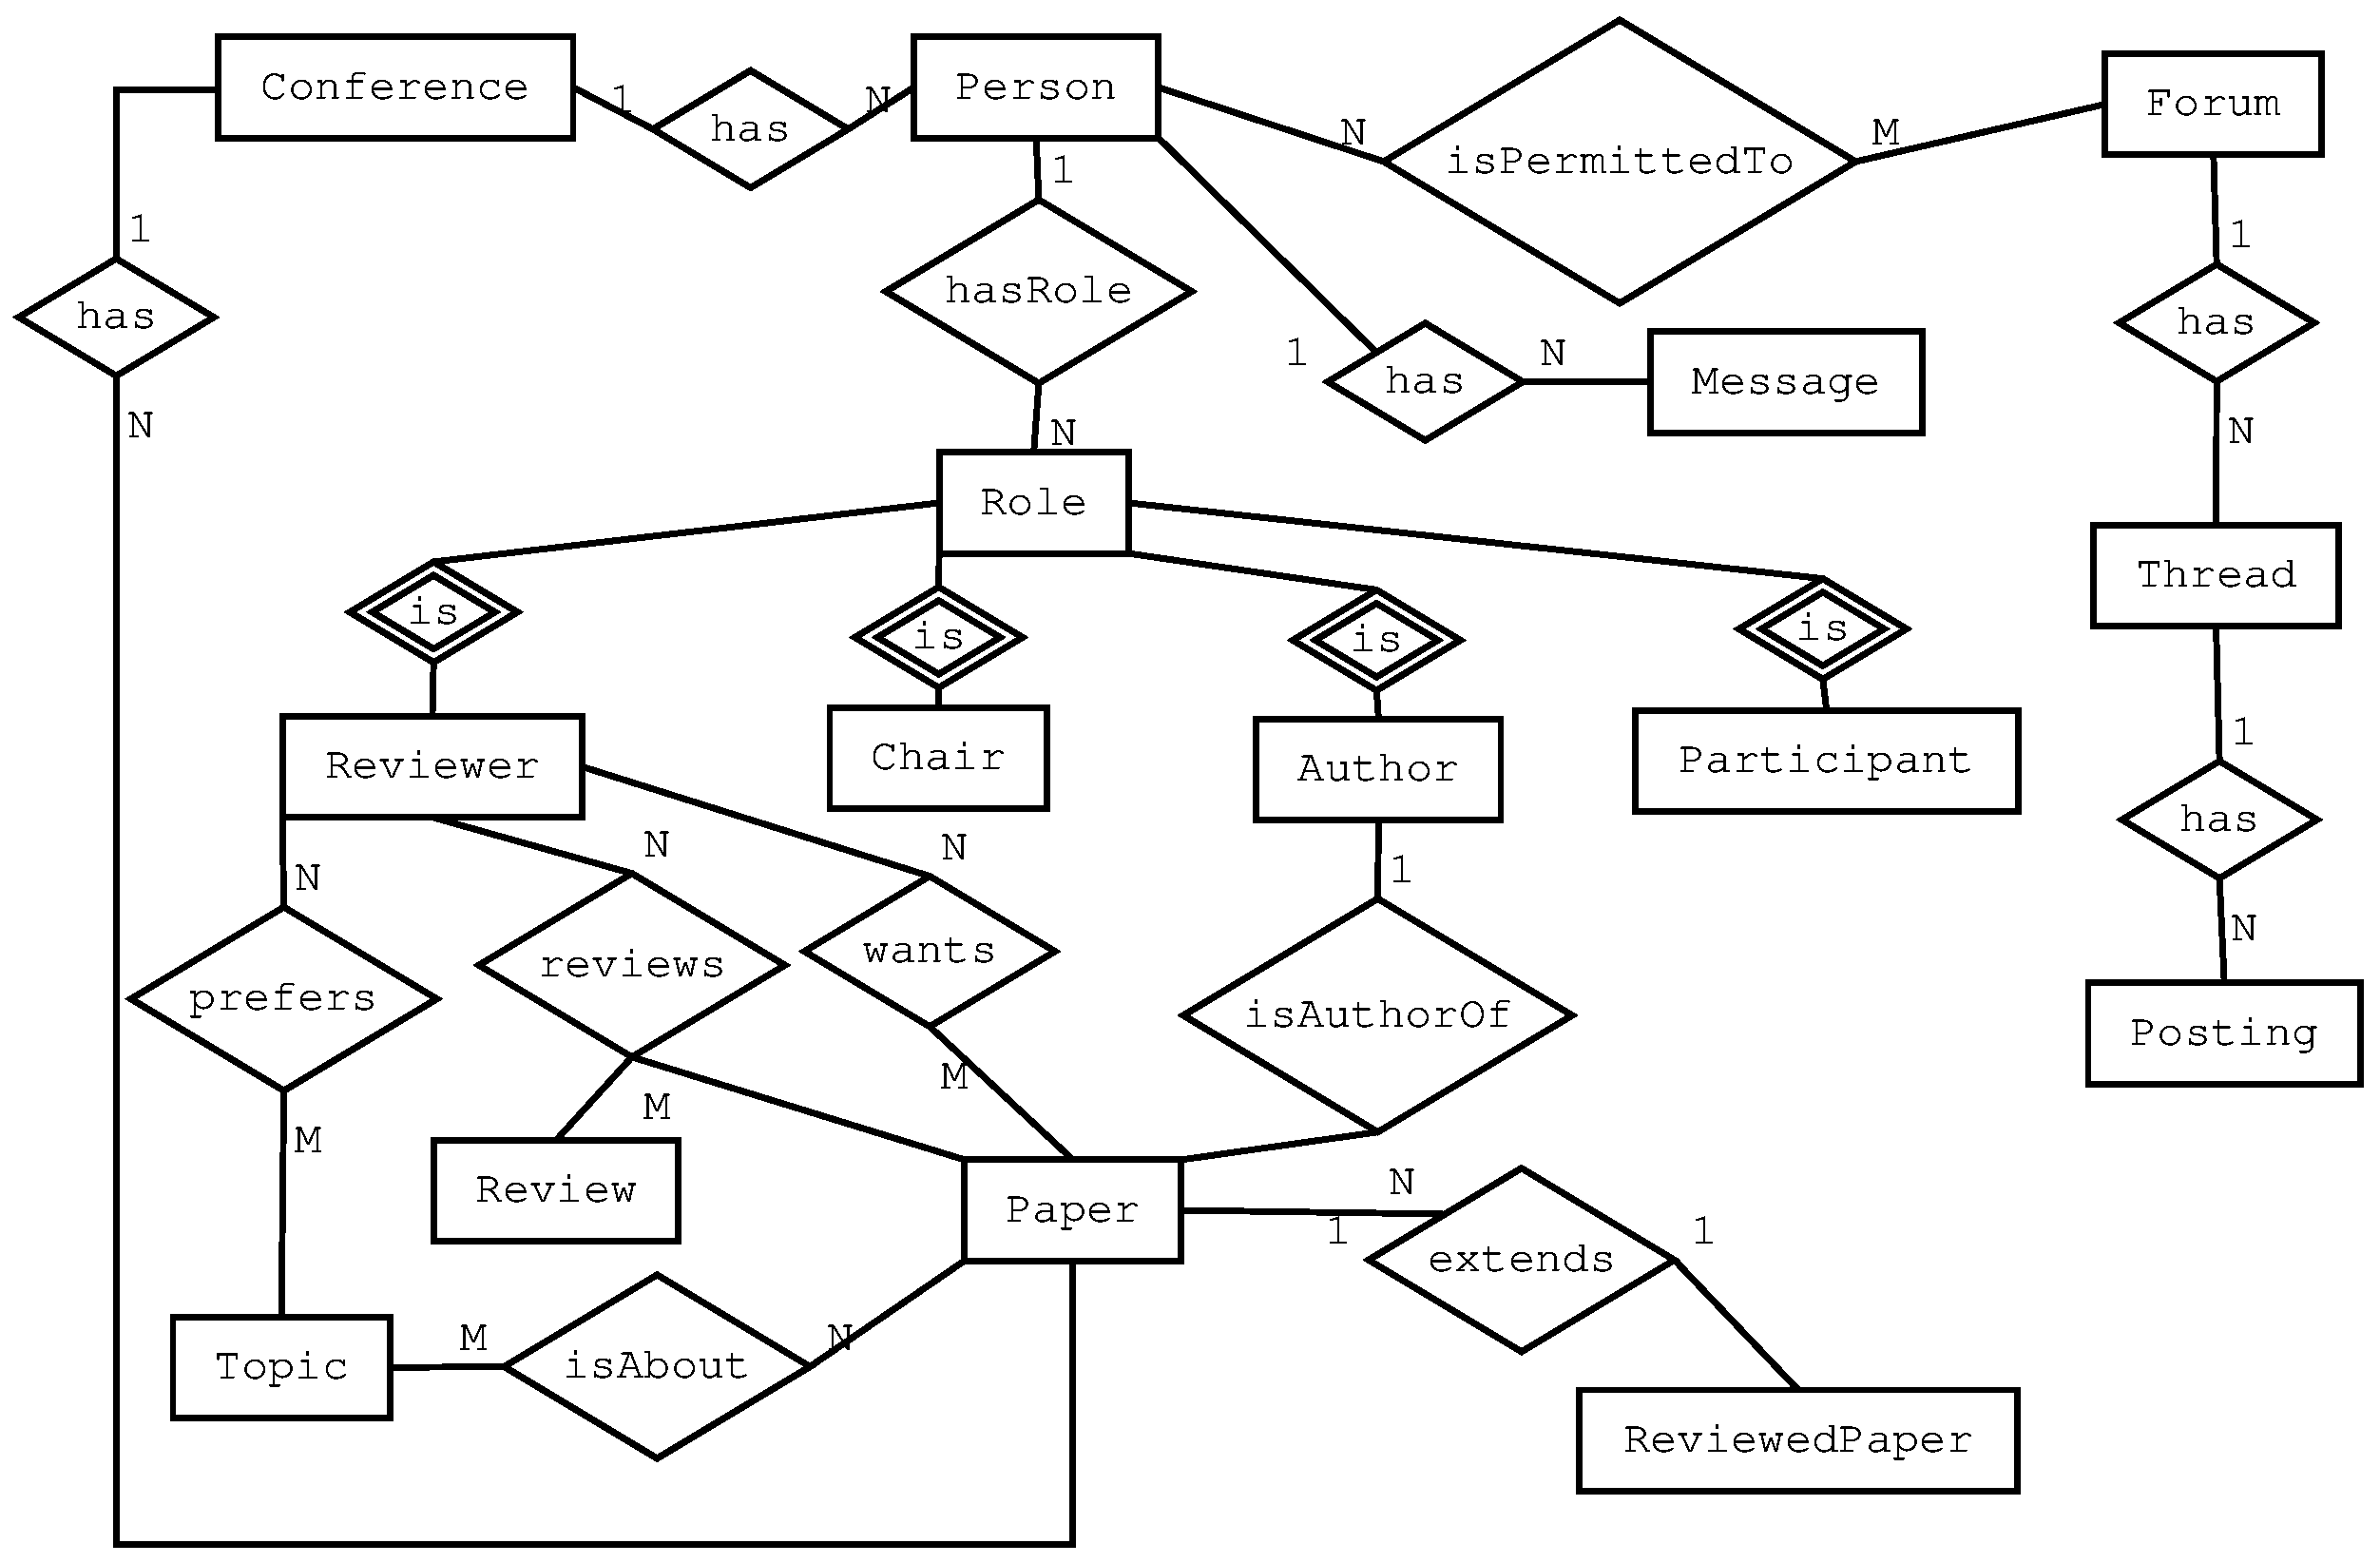
\includegraphics[width=15cm]{er-diagram}

    \begin{quote}
    W"ahrend das vorangegangene Kapitel das Datenmodell anhand der Objekte und ihrer Attribute
    beschreibt, soll das ER-Diagramm die Beziehungen zwischen den Objekten, insbesondere deren
    Kardinalit"aten verdeutlichen.
    \end{quote}

    \newpage

\end{document}
